\problemname{Reseplaneraren}

\noindent
Efter att ha åkt kollektivtrafik i flera år har du märkt att Bästtrafiks reseplaneringsapp inte är särskilt bra.
Ofta föreslår den rutter med 3 byten, när du vet att det går att göra resan utan några byten alls! För att visa
hur inkompetenta de är kommer du utveckla en konkurrerande app som avgör om man kan resa från station $A$ till
station $B$ utan några byten alls.

Göteborgs kollektivtrafiknätverk kan beskrivas utifrån dess $N$ hållplatser. 
Dessa hållplatser förbinds av ett flertal vägar. Nätverket av vägar är utformat så att man kan resa mellan varje
par av hållplatser, och det innehåller exakt $N-1$ vägar. 
Detta innebär att vägnätverket bildar ett träd. 
I ett träd definieras en stig som en följd av hållplatser där varje hållplats är direkt ansluten till nästa i följden,
och ingen hållplats passeras mer än en gång. Stigen mellan två hållplatser är alltid den kortaste och den enda möjliga
stigen som förbinder dem. Kollektivtrafiken utgörs av $K$ stycken spårvagnslinjer som åker i nätverket. Varje linje har
en spårvagn som åker mellan två stationer, start och slut. Denna spårvagn åker fram och tillbaka mellan start
och slut om och om igen. Vägarna har nog med spår för att spårvagnarna aldrig kan fastna eller hamna i kö.

Din app ska nu svara på $Q$ stycken frågor på formen: ''kan man åka från station $a$ till station $b$
utan byten''? Det vill säga, kan du hoppa på en spårvagn vid station $a$, låta spårvagnen åka en stund och sen
hoppa av vid station $b$? För att kunna håna Bästtrafik så mycket som möjligt så bryr du dig inte alls om hur
lång resan tar.

\section*{Indata}
Den första raden i indatan innehåller heltalen $N, K$ och $Q$ ($1 \le N, K, Q \le 3 \cdot 10^5$), antalet stationer,
spårvagnslinjer och frågor.

De följande $N-1$ raderna innehåller vardera heltalen $u,v$ ($1 \leq u,v \leq N$, $u \neq v$),
vilket betyder att det finns en väg mellan station $u$ och $v$. 

Därefter följer $K$ rader som vardera innehåller heltalen $s,t$ ($1 \leq s,t \leq N$, $s \neq t$), vilket
betyder att det går en spårvagn mellan station $s$ och $t$.

De sista $Q$ raderna innehåller vardera heltalen $a,b$ ($1 \leq a,b \leq N$, $a \neq b$), vilket
representerar en fråga om man kan åka från station $a$ till station $b$ utan byten. 

\textbf{Notera} att detta problemet har väldigt mycket indata. Det är därför rekommenderat
att använda snabb indataläsning.

\section*{Utdata}
För varje fråga, skriv ut ''Yes'' om man kan utföra resan utan byten, annars
''No''. Skriv ut dessa i samma ordning som indatan.

\section*{Poängsättning}
Din lösning kommer att testas på en mängd testfallsgrupper.
För att få poäng för en grupp så måste du klara alla testfall i gruppen.

\noindent
\begin{tabular}{| l | l | p{12cm} |}
  \hline
  \textbf{Grupp} & \textbf{Poäng} & \textbf{Gränser} \\ \hline
  $1$    & $7$       & $N, K, Q \leq 100$ \\ \hline
  $2$    & $19$       & $N, K, Q \leq 1000$. \\ \hline
  $3$    & $13$       & $N, K, Q \leq 5 \cdot 10^4$ \\ \hline
  $4$    & $23$       & För varje fråga befinner sig $a$ på stigen mellan $1$ och $b$. \\ \hline
  $5$    & $38$       & Inga ytterligare begränsningar. \\ \hline
\end{tabular}

\section*{Förklaring av exempelfall 1}
\begin{figure}[h]
  \centering
  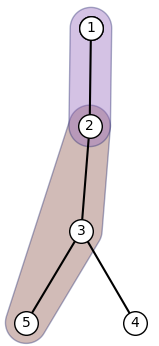
\includegraphics{sample.png}
  \caption{Visualisering av exempelfall 1. De svarta kanterna är vägarna, och de färgade områdena representerar
  vardera en spårvagnslinje.}
  \label{fig:exempelfall1}
\end{figure}

\begin{itemize}
  \item Fråga 1: det går inte att åka från station 1 till station 3 utan ett byte. Om man fick byta en gång hade det gått.
  \item Fråga 2: det går inte ens en linje till station 4, så då går det verkligen inte att göra resan utan byten.
  \item Fråga 3: här kan vi ta linjen mellan station 1 och 2.
  \item Fråga 4: här kan vi ta linjen mellan station 5 och 3.
\end{itemize}
